
\chapter{Transmission biases}
\label{Transmission biases}



Anyone who wants a natural, causal account of linguistic and other cultural transmission will have to study transmission biases.\is{transmission biases} These are the biases that ultimately regulate the historical, cumulative transmission of culture. To understand how the linguistic habits of communities change over generations --- in a diachronic frame\is{diachronic frame} --- we must also look in the ontogenetic frame,\is{ontogenetic frame} that is, in the process of language acquisition,\is{first language acquisition} and the resultant slight differences in habits of speech between generations. Language acquisition involves the effective transmission of a language from parents to children. Imperfections in this transmission are sometimes thought to explain language change.\is{language change} Consistent patterns in the details of such changes have been documented across a wide range of the world's languages. Many to argue that natural paths of semantic change are motivated by species-wide innate conceptual structure. There are universals\is{universals} in semantic change,\is{semantic change} independent from social factors and other factors outside the minds and bodies of speakers. But this is only part of the story. Even when new ideas for ways of saying things have their source within a single person, the spread of that idea follows mechanisms of population-level social transmission. And the success or failure of such transmission is ultimately dependent on the biases that are the topic of this chapter.

Cultural transmission can be usefully understood in relation to epidemiology\is{epidemiology} \citep{sperber_anthropology_1985}. We catch ideas from others, in this case ideas for attributing meanings to signs.


\begin{quotation}
	An innovation\is{innovation} in a language begins its existence in the mouths and minds of one or more speakers and spreads from them to other speakers. In fact, innovations occur constantly in the speech of individuals, but an innovation becomes part of the history of the language only when it spreads through the network to become a stable feature in the speech of a group of speakers. \citep[214-5]{ross_social_1997} 

\end{quotation}
	
	On syntax specifically, Harris and Campbell make a similar point:

\begin{quotation}
	Isolated creative, exploratory expressions are made constantly by speakers of all ages. Such expressions may be developed for emphasis, for stylistic or pragmatic reasons (to facilitate communication as in changes to avoid ambiguity or to foster easier identification of discourse roles), or they may result from production errors. The vast majority of such expressions are never repeated, but a few \textquoteleft catch on'. \citep[54]{harris_historical_1995}
\end{quotation}

\textit{How} do they catch on? How do they make this leap from single speaker to population-wide? How does an innovation become a stable feature in the speech of a group of speakers? In this chapter I discuss a crucial part of the answer to this question: the \textit{biases} that operate in linguistic and cultural change, in the diachronic frame.\is{diachronic frame} I will define some important biases, and I will say why we need a coherent conceptual framework to explain just why we observe the biases we observe. 


\section{Cultural epidemiology}
\is{epidemiology}

In the cultural evolution of language, that is, the diffusion, 
maintenance, and change of linguistic practices in historical 
communities, it is often assumed or implied that the unit of analysis is 
the language system as a whole.\is{languages, as unit of analysis} But the diachronic\is{diachronic frame} replication and transmission of 
whole language systems is not causally conducted directly at the system level (see Chapter \ref{causalunits} above). It 
is an aggregate outcome of a massive set of much simpler and much 
smaller concrete speech events that operate, in enchronic and microgenetic frames,\is{microgenetic frame} on the \textit{parts} of a language, such as words or pieces of grammar\is{linguistic items} 
\citep{hudson_sociolinguistics_1996}. 



Language systems only exist because populations of linguistic items 
replicate and circulate in human communities, whenever people say things. A causal account of language evolution\is{evolution!of languages} that focuses on the transmission of linguistic items can be called an 
epidemiological view, following \citet{sperber_anthropology_1985,sperber_explaining_1996}, 
and in a similar spirit to \citet{keller_language_1994} and \citet{croft_explaining_2000}. In an 
item-based account, the pieces of a system 
can change independently from other pieces, and they can be plucked out 
and borrowed from one system to another. This happens for example when we borrow a 
word. In diachronic\is{diachronic frame} processes, both enchronic\is{enchronic frame} and microgenetic\is{microgenetic frame} processes play a role.



Ultimately we need a causal account for why it sometimes seems like we 
can treat languages as if they were organism-like systems (e.g., when we 
write grammars). This is the topic of Chapter \ref{itemsystemproblem}, below. But first we need to define the basic underlying causal anatomy of item-based 
language transmission. Here I outline the basics of a transmission 
biases\is{transmission biases} approach to the historical evolution of languages. 



\section{Biased transmission}


The diffusion of cultural items in the diachronic frame\is{diachronic frame} is explained in terms of a \textit{biased transmission} model of the distribution of cultural knowledge 
and practice within human populations and across generations, following 
a general framework of cultural epidemiology\is{epidemiology} \citep{sperber_anthropology_1985,sperber_explaining_1996,boyd_culture_1985,boyd_origin_2005,enfield_linguistic_2003,enfield_transmission_2008}. In a biased transmission model, the question of whether 
fashions of cultural practice in a population spread, decline, 
transform, or remain as they are will be determined the cumulative 
effect of biases: filters, pumps, and transformers 
on cultural practices in a competition for social uptake. The processes are visible in the diachronic frame,\is{diachronic frame} but their proximal causal bases are seen in enchronic\is{enchronic frame} and microgenetic frames.\is{microgenetic frame}



Linguistic and other cultural items are not confined to the mind. Nor are they confined to things or actions that can be perceived. They are simultaneously manifest in mental \textit{and} 
material domains, \textit{and} in relations between these domains. At 
any moment, a community is buzzing with enchronic and microgenetic causal chains that constitute continuous lines of 
production and comprehension of pieces of language and culture. I am 
referring to people's courses of goal-directed action using words, tools, body movements, 
and other cultural items. 



These courses of behaviour are contexts in which the natural 
histories of cultural and linguistic items are played out. They 
constitute causal chains with links from mind (I know a word, I 
understand a tool) to usage (I use the word in conversation, I 
use the tool for a purpose), to mind (the other person learns or recognizes 
the word, an onlooker learns or recognizes the tool's 
function, attributing a goal to my behaviour), to usage, to mind, to 
usage, to mind, to usage, and so on. This type of causal 
trajectory is a chain of \textit{iterated practice},\is{iterated practice} or a cognitive 
causal chain\is{cognitive 
causal chain} \citep{sperber_why_2006-1}. See Figure \ref{iteratedpractice} for a simplified illustration.





\begin{figure}[h]
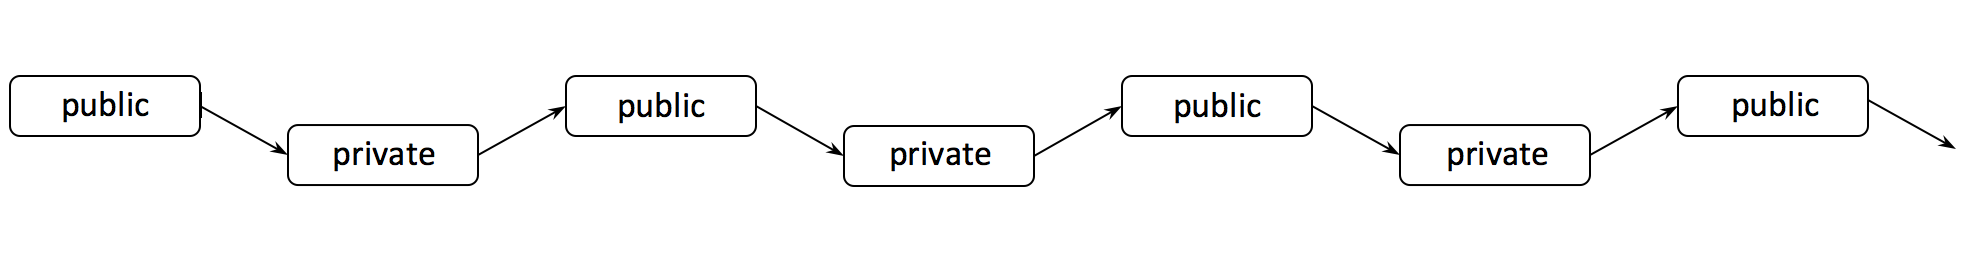
\includegraphics[width=0.95\textwidth,keepaspectratio]{figures/ch02fig01}
\caption{Simplified illustration of iterated practice, or a social 
cognitive causal chain (Sperber 2006:438).}
\label{iteratedpractice}
\end{figure}



Figure \ref{iteratedpractice} is not an \textit{iterated learning} chain,\is{iterated learning} of the kind presented by 
Kirby and colleagues \citep{kirby_ug_2004,kirby_cumulative_2008}, among 
others (\citealt{christiansen_language_2008}; see below). Those iterated learning depictions resemble Figure \ref{iteratedpractice}, 
but they are not the same. In iterated learning (studied to date using small, artificial languages in lab settings), each arrow from public 
to private may represent an entire learning process in an ontogenetic frame,\is{ontogenetic frame} such as a child's 
learning of a language.\is{first language acquisition} Each link in the chain is effectively a single 
macro-level state change in ontogeny (e.g., the move from not knowing 
the language to knowing the language). This is shorthand for a huge set 
of small events and small associated state changes. 



Learning a language involves not one event but many iterations of 
exposure and reproduction. In each micro-occasion of exposure and 
reproduction there is feedback that comes from others' reactions to how we use words in context. This feedback\is{feedback} plays 
an essential role in learning. Both the microgenetic\is{microgenetic frame} and ontogenetic frames\is{ontogenetic frame} are relevant. The iterated learning\is{iterated learning} model abstracts 
away from these details (not without practical reason), while the 
iterated practice\is{iterated practice} model in Figure \ref{iteratedpractice} tries to capture them directly and 
explicitly. 



While iterated learning focuses on the ontogenetic\is{ontogenetic frame} or biographical 
frame, iterated practice focuses on the enchronic 
frame,\is{enchronic 
frame} that is, the frame of moves and counter-moves in 
human interaction\is{social interaction} (see \citealt[10]{enfield_anatomy_2009}, \citeyear[Chapter 4]{enfield_relationship_2013}). In \ref{iteratedpractice}, each link in the chain from 
private-public-private does not represent a generation of individuals in 
a human population (by contrast with the comparable figure in 
\citealt{christiansen_language_2008}). It represents a generation of individuals 
in a population of items,\is{linguistic items} that is, one local cycle of 
instantiation of a practice, such as a single use of a word, a single 
performance of a ritual, or a single occasion of making bacon and eggs 
for breakfast. 



The schema in \ref{iteratedpractice} draws our attention to a set of bridges that a bit 
of culture has to cross if it is to survive a cycle of iterated 
practice.\is{iterated practice} What are the forces that help things across those 
bridges, and what are the forces that inhibit them? These forces are 
called transmission biases (following \citealt{boyd_culture_1985,boyd_origin_2005}). 
This kind of account assumes a standard model of Darwinian\is{Darwin} 
evolution\is{evolution} --- variation of heritable traits in a population --- where 
the variation\is{guided variation} is guided in a specific way. 



As \citet{boyd_culture_1985} formulate it, variation of cultural items 
is guided by the properties of people. For example, if a certain 
way of doing something is easier to learn than some other functionally 
equivalent way (e.g., doing mathematics on a calculator versus on an abacus), 
then this is likely to increase the frequency of the easier 
variant in the population. All things being equal, this variant 
will also in turn become more frequent simply because it is already 
more frequent. 



\citet{christiansen_language_2008} use this idea in arguing that the 
properties of the human brain, e.g., for learning and 
processing language, favour certain linguistic variants over others. Language is the way it is because it is \textquoteleft shaped by the 
brain', and thus not because the evolution of a language faculty\is{language faculty} has 
caused the human brain to change in some fundamental way as a result of 
the way language is. 



Assuming this model of guided variation, the question then becomes: What 
are the forces that guide variation in this way, and that 
operate upon variants within a population, ultimately 
determining whether those variants become, or remain, conventional in the 
population? We now consider some known biases.



\section{Some known biases}
\label{someknownbiases}

Variants of cultural behaviour compete for adoption by people in populations. Different researchers have described different 
biases, sometimes in quite specific terms, sometimes in broader terms. 



Christiansen and Chater (\citeyear{christiansen_language_2008}; see also \citealt{chater_language_2010}) describe four factors that mostly have to do with properties of the 
individual human body, especially the brain. These are (1) perceptuo-motor 
factors, (2) cognitive limitations on learning and processing, (3) 
constraints from mental representations, (4) pragmatic constraints. 
These factors can affect the likelihood that one linguistic variant is 
selected over another. (The social mechanisms that are also a 
necessary part of the process are left implicit by these authors.) 



\citet{boyd_culture_1985} introduce distinctions that are 
broader in kind. They illustrate with an example from table tennis.\is{table tennis} For 
the function of hitting the ball, you can choose between holding the bat 
with a pencil grip or a handle grip. Choosing one of these variants 
necessarily rules out choosing the other. They discuss biases 
that might cause a person to select one or the other grip. 



A \textit{direct bias}\is{transmission bias!direct bias} has to do with the relationship between a variant 
and a person who adopts that variant. It concerns affordances\is{affordances} \citep{gibson_ecological_1979}. A person should choose variant A if it is somehow more advantageous 
than variant B for a proximate function in some context. By a 
direct bias we should choose the grip that is easier, more effective, 
feels better, gives better results. 



An \textit{indirect bias}\is{transmission bias!indirect bias} has to do with social 
identity. When a person adopts a variant, other people will see. This will lend a certain status to both the adopter (as 
the kind of person who adopts that variant) and the variant (as a 
variant that is adopted by that person or someone like that). People adopt 
variants of behaviours not only for their efficacy but also 
with some idea of how they will be seen by others when they make that 
choice. So by an indirect bias we should choose the same grip as people 
who we identify with, or want to emulate. 



Finally, a \textit{frequency-dependent bias} favours variants that are 
more frequent.\is{transmission bias!frequency-dependent bias} 



Similar biases have been described in a large literature in sociology on 
the diffusion of innovations\is{innovation} (Rogers 2003). Here, we can discern three 
sets of conditioning or causal factors in the success or failure of a 
practice. 

\begin{enumerate}
\item \textit{Sociometric factors}\is{sociometric factors} have to do with the network structure of 
demographic groups. People are socially 
connected in different ways, especially in terms of the number of their points of 
connection to others in a social network, as well as the quality of these connections. A practice is more likely to spread if 
it is modelled by someone who is widely connected in a network. This is because he or she will expose a greater number of people to the 
practice. \citet{gladwell_tipping_2000} refers to this as the law of the few: a small number of people in group have the biggest influence on the diffusion of innovation. 



\item \textit{Personality factors}\is{personality factors} have to do with differences between 
people in the population that can affect the success 
or failure of an innovation. Some people are more willing than others to 
innovate and to adopt others' innovations (early adopters versus 
laggards). These differences may correlate with social categories 
such as age, class, and sub-culture. Some people are better known or 
better admired in their social milieu and may thus be more likely to be 
imitated. 



\item The \textit{utility}\is{utility} of an innovation is more or 
less what \citet{boyd_culture_1985} refer to as direct bias,\is{transmission bias!direct bias}  outlined 
above. The innovation will take off if it is more advantageous to 
potential adopters. 
\end{enumerate}



Each of the biases we have just reviewed plays an important 
role in the mechanisms of transmission that drive the circulation of 
bits of culture in human populations. But how to explain them? Where do 
these biases come from and how are they related to each other? Can we motivate these biases by 
locating them directly in the causal anatomy of transmission?  


\section{A scheme for grounding the biases}


One way to justify and limit the number of transmission 
biases is to motivate them in terms of the structure of iterated practice\is{iterated practice} shown in Figure \ref{iteratedpractice}. This structure gives us a way of locating and characterizing the biases. 
If we look at the elements of transmission illustrated in Figure \ref{iteratedpractice}, we see 
at the heart of it a repeating, four-stroke cycle consisting of the following steps: 


\begin{enumerate}
 
\item \textit{Exposure}:\is{exposure} a process of going from public (out in the world) to private (in someone's mind), 
when a person comes into contact with, and 
perceives or engages with, a bit of culture;



\item \textit{Representation}:\is{representation} how an idea is created and stored in the mind, based on (1), and the private product of this process;



\item \textit{Reproduction}:\is{reproduction} a process of going from private (in someone's mind) to public (out in the world), 
made possible in part by a person's motivation to cause the same 
public event as in (1). 



\item \textit{Material}:\is{material} the physical result of an 
event of reproduction of a cultural item.



\item Stages (3-4) can then lead to another round by exposing another 
person to the cultural item in question (feeding into a new stage (1)). 

\end{enumerate}





\begin{figure}[h]
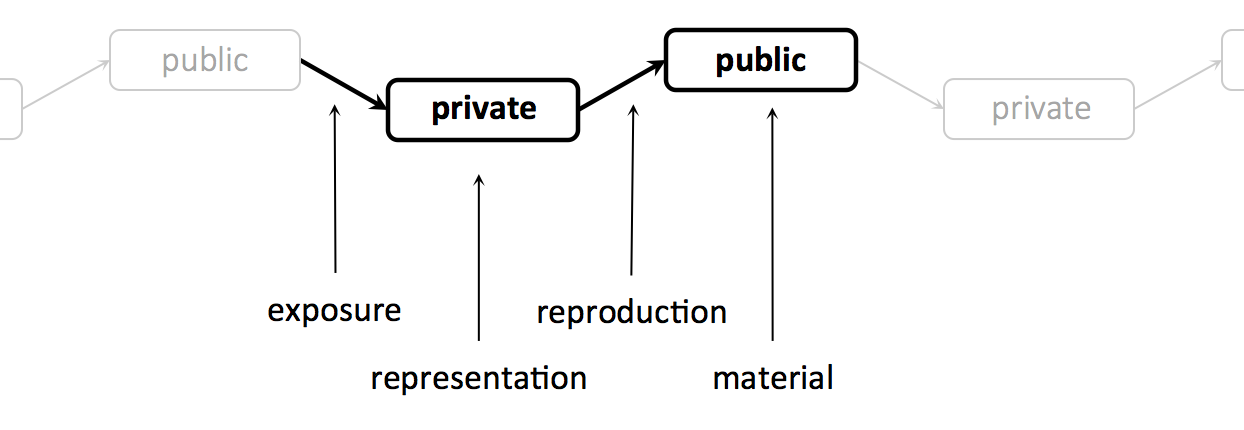
\includegraphics[width=0.95\textwidth,keepaspectratio]{figures/ch02fig02}
\caption{Loci for transmission biases; a four-stroke engine model.}
\label{fourstroke}
\end{figure}




Each of the four steps is a possible threshold for any bit 
of culture to succeed or fail in the competition for uptake in a community. If people aren't exposed to it, it will die. If it is 
difficult to remember or think of, or if in the course of mental 
representation it is radically altered, it will die, or effectively die. 
If people aren't motivated to reproduce it, no further exposure will 
happen, and when the people who have learned the practice in question die, the practice will die with them. This happens for example with language 
extinction. And if the practice is not physically realized, so that others may perceive it, the transmission process will 
stall. 



Failure on any of these four loci of transmission causes a break in the 
chain and may cause the variant to no longer exist. 



Do not get the impression that a single such chain 
represents the entire historical trajectory of a cultural item. It is 
only the tiniest strand. At any moment, there is a thicket of equivalent 
chains of iterated practice that keep a bit of language or culture alive and evolving in 
a community. 



Again, the question that a biased transmission approach 
to linguistic epidemiology asks is: What are the filters, 
pumps, and transformers that act upon the history of a cultural item? On the present proposal, we 
can posit four functionally-defined loci at which any bias can have an 
effect. Each locus is defined by the function it serves in braking, accelerating, or altering the transmission of practices in communities 
through social-cultural interaction, in an enchronic frame. 



While there may be a long, if not open list of possible biases, they all 
should be definable in terms of how they operate upon one or more of the four 
transmission loci, exhaustively defined by the causal structure 
represented in Figures \ref{iteratedpractice} and \ref{fourstroke} above: \textit{exposure} (world-to-mind transition), 
\textit{representation} (mind structure), \textit{reproduction} (mind-to-world 
transition), and \textit{material} (world structure). Within the framework of 
these basic causal loci for transmission (1-4), different biases may affect the transmission of a practice in different ways. 



As sketched above, some of these biases will have to do with facts about 
social networks, some with individual personality traits, some with 
properties of human perception, attention, memory, and action, some with 
the shape of the human body, some with the culture-specific means and 
ends that come with culturally evolved structures of activity, some with 
the organization of complex information in cognition. Let us now briefly 
consider how the previously described biases fit within 
the framework of these minimal loci for cultural transmission. Before we start, here is an important point. The goal of this exercise is not to locate each bias at just one point in the chain. As we shall see, some biases have effects at more than one point. This is one of the things the exercise shows us.


\subsection{Exposure}
\is{exposure}
Exposure --- relating to the world-to-mind transition --- is where 
biases can affect the likelihood that a person will come into contact 
with, and pay attention to, a practice.



One type of bias that effects exposure is social connectedness. All people are situated in social networks,\is{social networks} 
but they are situated in different ways. One type of difference between 
people has to do with the number of other people we come into contact with. 
\textit{Connectors} have a large number of social ties \citep{granovetter_strength_1973}. They are more likely to be exposed to an 
innovation, or to expose others to it. People with fewer social network connections will have a 
lower chance of being exposed to a given practice, or exposing others. 



Another type of bias relevant to exposure is salience.\is{salience}\is{transmission bias!salience bias}  When you come across a new kind of behaviour you may or may not pay attention to it. The things that stand out will more likely to attract your attention. The definition of \textquoteleft stand out' is 
clearly a matter of perception in the classical sense of affordances,\is{affordances} 
that is, a matter of the \textit{relationship between} a person and a thing being perceived. 
Some things are more likely to be noticed because of the nature of our 
senses in relation to the world. Other things are more 
salient to us because we are actively looking for them, often because our 
language or culture encourages or requires it.



A third bias relevant to exposure is identity.\is{identity}\is{transmission bias!identity bias}  Who is the person carrying out the practice when 
it is encountered? If it is somebody who I want to be like in some 
way, then I am more likely to pay attention to what the person is doing 
and how. If it is someone I have no interest in, I will be less likely to pay attention. In this way, social 
identity can play a role in biasing exposure, by affecting the extent to 
which someone will attend, or carefully attend, to the practice when 
encountered.


\subsection{Representation}
\is{representation}
Representation --- relating to mind structure --- is where biases can 
affect the likelihood that, or the manner in which, a practice will be 
learnt or stored by a person, or how the psychological or otherwise 
private component of a practice will be structured. 



Once we are exposed to a certain pattern of behaviour, we can 
learn it. We form a representation of it, attributing to it some meaning 
or function, and we incorporate that representation into an existing framework of knowledge. 



Some innovations\is{innovation} are more memorable than others. Some things are more easily internalized. This is explained by cognitive preferences that are either known from 
psychological science or that are on that research agenda. 



There are other differences in how things are learnt. Whether you see a thing, hear it, feel it, or some combination of these, can have 
consequences for how that thing is interpreted, learnt and understood 
\citep[Chapter 6]{enfield_anatomy_2009}. This can then affect how the new knowledge is applied. For example, it may shape how you decide that a practice 
is an appropriate means for certain ends in a particular context.



There are effects of the psychological context into which a practice is 
embedded. Practices are partly constituted by knowledge; knowledge that 
is caused by, and in turn causes, public behaviour and associated states 
of affairs. Knowledge has structure, including part-whole relations, hierarchical 
relations, and other sorts of dependency among items in a system. 



When we learn something,\is{learning} we relate it to other things we know. We do this at the 
very least because the thing stood in a certain relation to other things in the context 
in which we learnt it. As an example, if I learn a new word such as 
\textit{deplane}, I relate it to other words I already know. There might be similarities with other words: \textit{debone, derail, decode, decommission}. Or associations with other features of the language system: \textit{deplane} is a verb and 
can be used only with specific grammatical roles in English sentences.\is{English} 
Or if I learn about the possibility of downloadable ringtones I will 
naturally link this to my existing knowledge of mobile 
phones and the Internet. All of these are examples of a \textit{context bias}. Through a context bias\is{transmission bias!context bias}  a person is more readily able 
to learn and psychologically represent those things that have an 
existing \textquoteleft place' in which to fit. 



In language, items are structured into paradigms, syntagms, conceptual frames, semantic fields, and other kinds of linguistic systems.\is{systems} While these systems often display a degree of symmetry, 
consistency, and simplicity, change is always taking place. In a system, when something happens in one place 
this will have effects in another place. In lexicon and grammar, such system-internal 
dynamics\is{internal change} can give rise to a certain \textquoteleft psychological 
shakiness', as \citet{sapir_language:_1921} put it. As noted already in Chapter \ref{causaldynamics} above, this can lead to reorganization of 
a system, in people's heads, and then potentially in a whole community.



Now finally, note that \textit{content biases}\is{transmission bias!content bias}  are also relevant to the representation locus of transmission. In the broadest sense of meaning, capturing everything from the 
arbitrary meanings of words in languages to the affordance-grounded\is{affordances} 
functions of tools \citep{kockelman_residence_2006}, we benefit from what can be called 
natural meaning.\is{natural meaning} If a word or grammatical expression is compatible with 
other information, for example by having iconic properties, it is better 
learnt and remembered. Similarly for technology, if there is a good match between the intended function of a tool and the tool's natural affordances, then we are more likely to understand the practice of using that tool, it 
will be easier to learn, and indeed what needs to be stored 
in the mind is reduced because the relevant information can 
stored materially \citep{norman_cognitive_1991}. These examples of the content bias pertain to learning, storage, and 
reduction of load on cognition. 


\subsection{Reproduction}
\is{reproduction}
Reproduction --- relating to the mind-to-world transition --- is where biases can affect the likelihood that a person who is exposed to a kind of behaviour will later do it themselves. One way to think of this sense of reproduction is whatever causes a 
person to turn the private representation of a practice into an action 
whose production and effects are then perceptible by others.



What motivates us to turn knowledge into action? Daily life involves 
goal-directed behaviour that is motivated by our beliefs and desires  
\citep{davidson_essential_2006,searle_intentionality:_1983,fodor_psychosemantics_1987}. I may want to get 
something done for which I need another person's cooperation. One way to do this is with language. I select certain words and 
grammatical constructions as tools for the job. Depending on my goals, I will choose
certain words and will thereby choose against all the other words I 
could have used. 



This is the competition among words and grammatical forms invoked in 
Darwin's \citeyear[60]{darwin_descent_1871} citation of Max \citet{muller_darwinism_1870}: \textquoteleft A struggle for 
life is constantly going on amongst the words and grammatical forms in 
each language'. The competition among different cultural practices 
operates in the same way. I have a goal. I have beliefs about 
how it can be attained. I have knowledge that allows me to act. I can foresee at least some effects of my actions. All this 
points to a powerful bias at the reproduction locus of transmission, concerning a person's functional needs, and the available means to those ends. 



The content bias,\is{transmission bias!content bias}  again, fits partly under this 
rubric. As discussed above, a content bias favours a practice that is 
more beneficial in some way to the person who selects it. Recall that a direct content bias applies when the benefit is 
greater functional payoff, or reduced cost, of the practice, in 
terms of its primary functional effects. In the table tennis\is{table tennis} example (see section \ref{someknownbiases}, above), a direct content bias\is{transmission bias!direct bias}  would favour the pencil grip 
if the pencil grip were lower in cost or greater in benefit than the 
handle grip --- that is, in terms of its efficacy for getting the ball back 
over the net and, ultimately, for winning matches. An indirect content bias\is{transmission bias!indirect bias} is also relevant to the reproduction locus of transmission: the choice to use the variant at all will have to do with the effects of whom you might show yourself to identify with (or against). There is an extensive literature on this in sociolinguistics.\is{sociolinguistics} Speaking English,\is{English} I might say \textit{guy} 
in one context and \textit{bloke} in another. Maybe there is 
a slight meaning difference between these two words, thus invoking a 
direct content bias. But these differences may be minimal compared to 
the effect of identifying myself with certain sub-cultural groups or 
kinds of social relationship by virtue of this choice between different 
word forms with near-identical meanings. 



Clearer examples concern pronunciation. Whether I choose to say \textit{working} or \textit{workin'} has more to do with who I identify with 
(an indirect bias) rather than the meaning I want to convey (a direct 
bias). In the cultural realm, both a Rolex and a Tagheuer will tell the 
time for a high price but the choice to wear one or the other may depend on whether you want to 
identify with Roger Federer versus Tiger Woods (or tennis 
versus golf). 



And there is perhaps most often some combination of the two. Do I choose 
to drink this brand of beer over all the rest because it tastes better 
(a direct bias) or because by doing so I identify with some person or 
group of people (an indirect bias)? It could be both. In any case, the 
mechanisms at play will bias a person's motivation for 
selecting one practice over all the others that he thereby does not 
select. 



The indirect bias\is{transmission bias!indirect bias} is also sometimes called a model bias.\is{transmission bias!model bias} An important distinction can be made here depending on the age 
of the person concerned. How does a child select which variants of a 
practice to adopt? A conformity bias\is{transmission bias!confirmity bias} favours those practices that 
`everyone else' adopts \citep{boyd_culture_1985,gergely_sylvias_2006}. Another term for this bias is docility\is{docility} \citep{simon_mechanism_1990}. This refers to an 
adaptive propensity to do what other 
members of your group do, and in the same ways, without wondering why. An infant's model group will tend also to 
consist of the people who she is genetically most closely related to. 
The effect is that cultural practices and genes tend to (but need not) have 
parallel histories. 

As people grow up and come to be regarded full members of their group, they come across a greater number and range of cultural items. They keep learning.\is{learning} So at any time they may 
find themselves with new choices. This may be because they 
encounter other ways of doing things than the way \textquoteleft my people' do things. This happens when they come into contact with other groups, for instance in trading, 
ritual and other kinds of inter-group social interaction.\is{social interaction} Different 
people in a community will have different degrees of mobility, sometimes as a result of 
personality, sometimes as a result of gender (men often travel more 
widely than women), age or sub-culture. 



At a later age, there is a greater degree of choice and therefore 
greater competition between choices. We may or may not consciously 
deliberate about such choices. But as adults we may be more aware of the 
meanings of different options. Here is where the indirect bias\is{transmission bias!indirect bias} looks 
more like the model bias\is{transmission bias!model bias} exploited in commercial advertising. This bias applies in 
all diffusional\is{diffusion} processes by favouring practices 
that are modelled by, for example, more admired or charismatic people.


\subsection{Material}
\is{material}
Material --- relating to world structure --- is where biases can 
affect the way in which a practice will be physically perceived. 



Biases on the material locus of transmission have to do with the physical affordances\is{affordances} of cultural practices, and the ways in which these affordances affect the exposure 
and reproduction of those practices. Material-related biases can affect exposure-related biases in some 
obvious ways. The material nature of speech is such that it fades almost instantly (gesture\is{gesture} slightly less so, etc; see \citealt{enfield_anatomy_2009}).
But when language is reproduced in writing,\is{writing} this evanescence is dramatically lessened, and the 
dynamics of transmission are significantly affected. 



Outside of language, we see similar contrasts. Many activities, like adopting a certain grip for table tennis,\is{table tennis} can only be seen momentarily. They are 
only available for exposure simultaneously with the reproduction process 
that potentially constitutes the transmission event (photos, etc., 
aside). The table tennis bat itself, however, has a more persistent 
physical existence, and can stand as a public sign for the possible ways people might handle it \citep{norman_design_1988,kockelman_residence_2006}. 



Material-related biases have to do with the ways in which cultural practices are made public, and how their form of public existence might affect their availability in the 
exposure-reproduction cycle we have been exploring here.

\subsection{Networks}
\is{social networks}
If the above-mentioned elements are an engine for the tranmission of innovation, then social networks are the paths that innovations take. The career of an idea may theoretically be mapped in a large but finite network (\citealt{luce_connectivity_1950}, \citealt[Chapter 12]{miller_language_1951}, \citealt{milroy_language_1980,ross_social_1997}). 

In fashion and other kinds of social epidemic, the success of an innovation\is{innovation} will partly depend on the ways in which people's personalities\is{personality factors} differ. As \citet{gladwell_tipping_2000} accessibly lays out, different personality types contribute to the diffusion of innovation in complementary ways. Connectors have a high number of weak social connections, in a range of social spheres. Mavens are actively interested in the market, and want to share their knowledge and opinions. Salesmen are the charismatic, persuasive ones who model innovations and effectively sell them. Innovators are the risk-takers who try things before anyone else does. They are followed by early adopters, the early majority, the more conservative late majority, and finally, the laggards.

When all of these types of people come into contact, they form social networks. The approach to language in terms of networks was pioneered in sociolinguistics\is{sociolinguistics} by \citet{milroy_language_1980}, and also taken up by \citet{le_page_acts_1985}, \citet{ross_social_1997}, and others. \citet{milroy_language_1980} developed a method for studying linguistic variation\is{variation} based around the idea of social networks, \textquoteleft the informal social relationships contracted by an individual' \citep[174]{milroy_language_1980}, which \textquoteleft can be used to account for variability in \textit{individual }linguistic behaviour in communities' \citep[21]{milroy_language_1980}. The social network model \textquoteleft treats speakers as nodes in a social network, such that each speaker is connected with other speakers by social (and therefore communication) links' \citep[213]{ross_social_1997}. The idea is to map the network of contacts that each individual has. Milroy suggested that networks could be placed on a scale of density, from low to high. In a low density network, \textit{a} may be in regular contact with \textit{b}, \textit{c}, and \textit{d}, but \textit{b}, \textit{c}, and \textit{d} are never in contact with each other. In a high density network, \textit{a}, \textit{b}, \textit{c}, and \textit{d} are all in contact with each other.

Usually, contacts between two people are made in the presence of other network members. So, to the high density network, we could add the ties \textit{a-b-c, a-b-d, a-c-d, b-c-d, }and \textit{a-b-c-d}.

The network concept contributes \textquoteleft to analysis of the manner in which individuals utilise the resources of linguistic variability available to them.' \citep[175]{milroy_language_1980}. In work with Li on the topic of code-switching, Milroy writes:

	\begin{quotation} (A) network analysis can... form an important component in an integrated social theory of language choice. It links the community with the interactional level in focusing on everyday behaviour of social actors. ...  The link with the economic and sociopolitical level derives from the observation that networks seem to form not arbitrarily but in response to social and economic pressures. \citep[155]{milroy_social_1995}
	\end{quotation}
	
While \textquoteleft density' refers to the intensity of contact among network members, there are distinctions in the quality of relationships between any two network members. A distinction between \textit{exchange} and \textit{interactive} networks was suggested by \citet{milardo_families_1988}, to which Milroy and Li add \textit{passive} network ties:

\begin{quotation}
Exchange networks constitute persons such as kin and close friends with whom ego not only interacts routinely, but also exchanges direct aid, advice, criticism, and support --- such ties may therefore be described as \textquoteleft strong'.  Interactive networks on the other hand consist of persons with whom ego interacts frequently and perhaps over prolonged periods of time, but on whom ego does not rely for personal favours and other material or symbolic resources --- such ties may be therefore described as \textquoteleft weak'. An example of an interactive tie would be that between a shop-owner and a customer. In addition to exchange and interactive ties, we identified a \textquoteleft passive' type of network tie, which seemed particularly important to migrant families. Passive ties entail an absence of regular contact, but are valued by ego as a source of influence and moral support. Examples are physically distant relatives or friends. \citep[138-139]{milroy_social_1995}
\end{quotation}

The key point is that sociolinguistics and network analysis give us a valuable matrix in which a four-stroke diffusion engine operates, modulated as it is by transmission biases (see especially \citealt{rogers_diffusion_2003} for a rich review of cases and analyses of the diffusion of social innovation).

\section{Causal anatomy of transmission}



A causal explanation of linguistic reality must include the role of transmission biases in the diffusion of innovations in social networks. A good diachronic\is{diachronic frame} account of language change must be explicit about the proximal causal 
anatomy of the process, operating in microgenetic,\is{microgenetic frame} enchronic,\is{enchronic frame} and ontogenetic\is{ontogenetic frame} frames. Previous work has usefully identified and 
described transmission biases, but one might ask: Why these biases? What 
other biases might we predict are possible? How many might there be? 



We can answer these questions with reference to the basic, proximal causal anatomy of social transmission. It is powered by a four-stroke engine, a causal chain in the enchronic frame, from 
exposure to representation to replication to material instantiation, 
back to exposure and round again. A transmission 
bias is any force that serves as a filter, pump, or transformer for this 
process, with effects on any of the links in the potentially open-ended chain of iterated practice. 

A next step is to see how well we can explain the known and understood biases 
within this four-stroke engine framework, and to see what predictions can be made and tested. This should connect to research 
on the puzzle of how our species evolved\is{evolution!biological} the capacity for cumulative 
culture \citep{tomasello_cultural_1999}, a capacity that is strongly pronounced in humans but weak 
if present at all in our closest relatives, the other apes\is{apes} \citep{herrmann_humans_2007}. While we can readily assume that other animals are 
engaged in goal-directed courses of action, and that they select from 
among different means for fixed ends in both the social and material 
realms, their selection of means for ends is relatively less flexible 
than that of humans. What is the link to transmission biases? We might assume that a chimpanzee, say, will be guided in its selection 
of a behavioural strategy by a strong content bias, incorporating a 
basic min-max payoff logic: keep effort to a minimum while ensuring the desired outcome. But if its repertoire of strategies is, on 
the whole, not being acquired by learning from others --- but, say, learned by ritualization during the course of life, in an ontogenetic frame --- then transmission 
biases will have no traction. 

%To what extent do other apes possess the cognitive prerequisites for social transmission of the kind described here? While the biggest differences between us and them are known to be in social cognition, they are nevertheless intensely social species with textured societies. Many of the crucial cognitive and sociometric ingredients for biased transmission may have been in place before the evolution of our species, allowing the processes to kick in as soon as culture was being transmitted at all. 



%True reconstruction of the historical process probably a hopeless quest (Leach quote - history is not ‘irrelevant’, but ‘too difficult to put on paper’.)



 

\newpage
